\chapter{Progetto}
\label{sec:arch}

Alla luce delle considerazioni esposte sui dati e sullo sviluppo, tenendo in conto che riscrivere l'intero microservizio in Rust con Vulkan non è un'operazione banale (e comunque non ci sarebbero stati enormi benefici in termini di prestazioni), si è scelto di adottare un approccio ibrido e quindi di mantenere i kernel in CUDA e usare Rust per la parte web del microservizio. Questo permette di mantenere le prestazioni e il know-how di CUDA e di poter sfruttare l'ecosistema e la development experience di Rust. Inoltre, l'uso di Rust per la parte web permette di avere un sistema più sicuro e performante su CPU rispetto alla controparte C++, e soprattutto più portabile e facilmente mantenibile, grazie al suo sistema di gestione delle dipendenze e alla sua capacità di compilare codice per diverse architetture.


\section{Struttura del microservizio}


Il progetto ha una struttura di questo tipo:

\vspace{5mm}
\begin{lstlisting}[language=bash, caption=Directory del progetto, label=lis:tree]
$ tree .
.
|-- build.rs
|-- Cargo.toml
|-- lib
|   |-- libsolver.so
|   \-- solver.h
\-- src
    |-- main.rs
    |-- solver.rs
    \-- models.rs
\end{lstlisting}
\vspace{5mm}

Il file \textit{Cargo.toml} contiene le dipendenze del progetto e le configurazioni di compilazione. Il file \textit{build.rs} contiene il codice necessario per il linking della libreria dinamica \verb|libsolver.so| di CUDA e specifica l'header da cui recuperare i simboli per la compilazione con \textit{autocxx} \ref{lis:build_rs}. La cartella \textit{src} contiene il codice Rust del microservizio, in cui: il file \textit{main.rs} contiene il codice principale del microservizio, con le REST API, mentre \textit{solver.rs} contiene le funzioni Rust per interfacciarsi con la shared library di CUDA tramite FFI. Infine, \textit{models.rs} contiene le strutture dati necessarie per la computazione e per la comunicazione con i client.

\vspace{5mm}
\begin{lstlisting}[language=Rust, caption=build.rs, label=lis:build_rs]
use std::env;
use std::path::PathBuf;

fn main() {
    let manifest = env::var("CARGO_MANIFEST_DIR").unwrap()
    let manifest_dir = PathBuf::from(manifest);
    println!("cargo:rerun-if-changed=src/solver.rs");

    // Define path to resolve #include relative position
    let include_path = manifest_dir.join("lib");
    let cuda_path = manifest_dir.join("/usr/local/cuda/include");
    let mut b = autocxx_build::Builder
        ::new("src/solver.rs", [&include_path, &cuda_path])
        .auto_allowlist(true)
        .build()
        .unwrap();
    b.flag_if_supported("-std=c++17").compile("ms-solver");

    println!("cargo:rustc-link-search=lib");
    println!("cargo:rustc-link-lib=solver");
    println!("cargo:rustc-env=LD_LIBRARY_PATH={}", 
        manifest_dir.join("lib").to_str().unwrap());
}
\end{lstlisting}
\vspace{5mm}

\begin{figure}[ht]
    \centering
    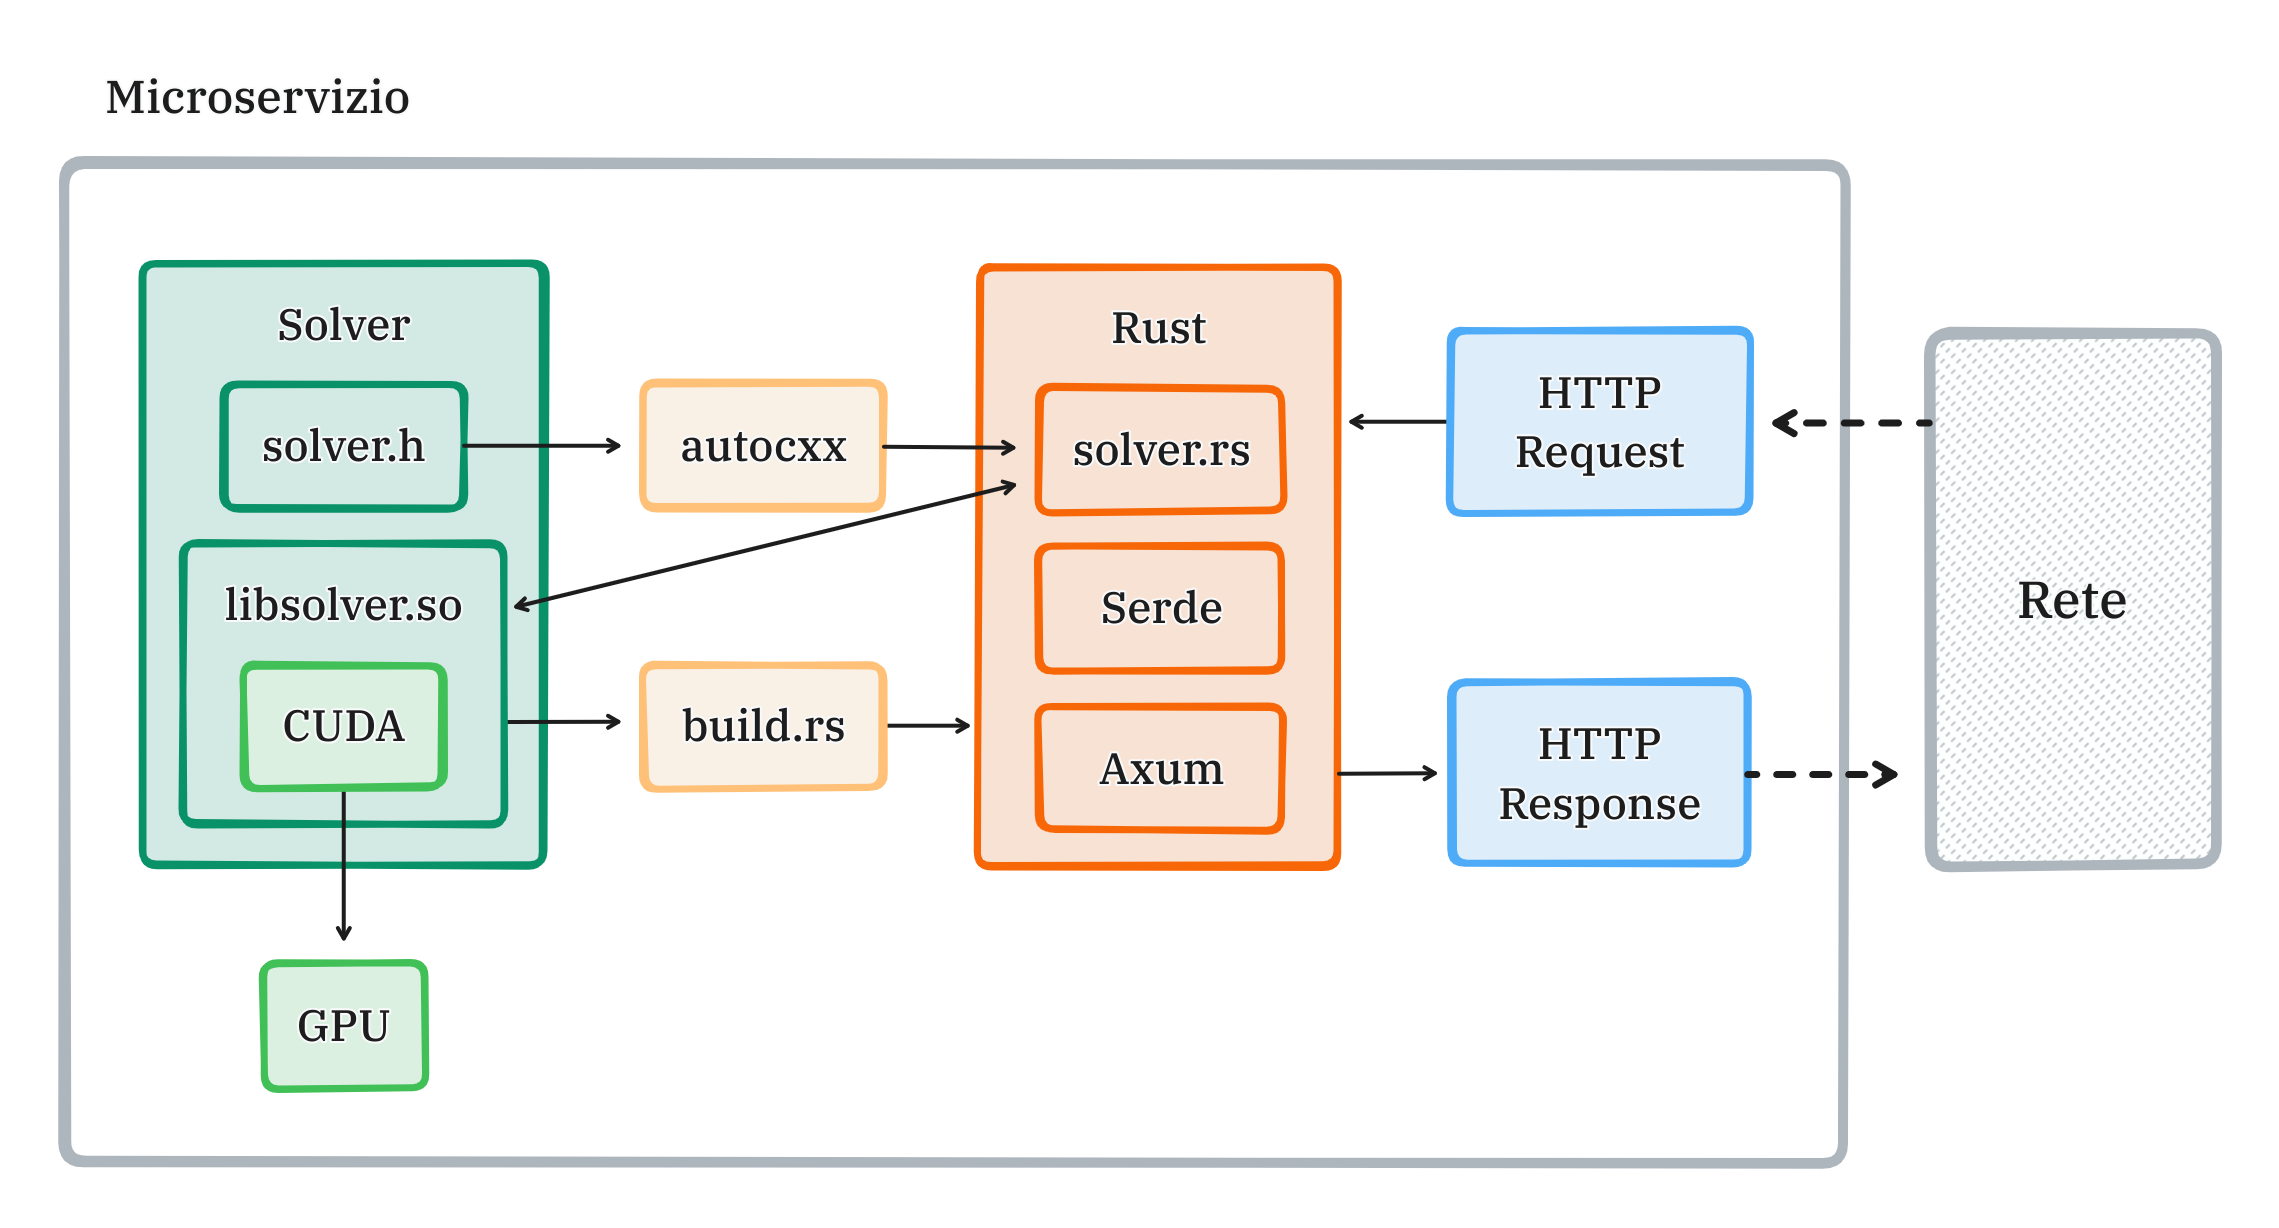
\includegraphics[width=1\linewidth]{images/chapter6/micro_arch.png}
    \caption{Architettura del microservizio}
    \label{fig:micro_arch}
\end{figure}


Per integrare Rust con la shared library di CUDA si è scelto di utilizzare al libreria \textit{autocxx} che, partendo dai file di header genera tramite marco il codice Rust necessario per interfacciarsi con la libreria. Questo permette di avere un codice Rust che è in grado di chiamare le funzioni della shared library di CUDA e di gestire i puntatori e le strutture dati necessarie per la computazione. Inoltre, \textit{autocxx} permette di gestire automaticamente la conversione dei tipi di dato tra Rust e C++, permettendo di scrivere codice Rust che è molto simile a quello C++.



\vspace{5mm}
\begin{lstlisting}[language=Rust, caption=Macro autocxx e uso della FFI, label=lis:generic_glsl]
// src/solver.rs

use std::ffi::{CStr, CString};
use crate::models::{Matrix, Model, QuboMatrix, Solutions};

autocxx::include_cpp! {
    #include "solver.h"

    safety!(unsafe_ffi)
    generate!("solve_matrix")
    generate!("health_check")
    generate!("get_device_count")
}
    
pub fn get_device_count() -> i32 {
    ffi::get_device_count().into()
}

pub fn health_check() -> String {
    unsafe {
        let ptr = ffi::health_check();
        let c_str = CStr::from_ptr(ptr);
        let c_string = CString::from(c_str);

        c_string.into_string().unwrap_or_default()
    }
}

pub fn solve_matrix(params: Matrix<f64>) -> Solutions<f64> { 
    ...
    unsafe { let _ = ffi::solve_matrix(params.qubo_matrix, ...); }
    ...
 }

// lib/solver.h

char const *health_check() { return "Hello from CUDA!"; }
int get_device_count();
int solve_matrix(...);
\end{lstlisting}
\vspace{5mm}



% spigare tokio
% spiegare axum
% spiegare rest api con json


\section{Piani futuri}

% sviluppo futuri con grpc di protobuf
% aggiunta test e CI ???